\documentclass[border=2mm]{standalone}
\usepackage[utf8]{inputenc}
\usepackage{pgfplots,tikz}

\begin{document}
      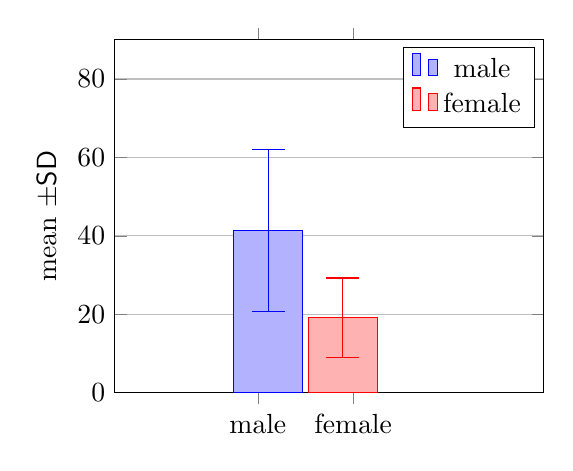
\begin{tikzpicture}
          \begin{axis}[
%		title=number of operations,
		width=200pt,
		xmin=0.96,xmax=1.05,
		xtick={0.99,1.01},
		xticklabels={male, female},
		ymin=0, ymax=90,
		ylabel={mean $\pm \mathsf{SD}$},
		ybar, 
            	bar width=25pt,			
		ymajorgrids,  						
		ylabel near ticks
	]


	
		\addplot+[error bars/.cd, error mark options={rotate=90, mark size=6pt},
			y dir=both, y explicit] coordinates{ (1,41.3) +- (0,20.61)};%41.3 is the mean, 20.61 is the SD
		\addplot+[error bars/.cd, error mark options={rotate=90, mark size=6pt},
			y dir=both, y explicit] coordinates{ (1,19.1) +- (0,10.12)};%19.1 is the mean, 10.12 is the SD

		\legend{male, female}
          \end{axis}
      \end{tikzpicture}
\end{document}
